\newpage
\mysubsection{Transaction}

\ifbook{

  \paragraph{} La plupart des applications en ligne ont généralement comme objectif de réaliser des
  \textbf{transactions}. On mesure d'ailleurs très souvent la performance d'un système au nombre de
  transactions effectuées par minute. La notion de transaction est donc au coeur de bien des aspects
  du \textbf{middleware}.

  \paragraph{} Bien que l'usage du terme \textbf{transaction} soit très répandu, son sens n'est
  forcément aussi clairement maîtrisé. En outre, chaque application a, dans les faits, sa propre
  définition et compréhension de la notion de transaction.

  \paragraph{} Nous allons donc commencer par étudier sa définition plus ou moins académique. D'après
  \mylink{http://fr.wikipedia.org/wiki/Transaction\_informatique}{Wikipédia} la définition d'une
  transaction (accédée le 27/12/2011) est la suivante:

  \paragraph{} \textit{En informatique, et particulièrement dans les bases de données, une
  transaction telle qu'une réservation, un achat ou un paiement est mise en oeuvre via une suite
  d'opérations qui font passer la base de données d'un état A - antérieur à la transaction - à un
  état B postérieur et des mécanismes permettent d'obtenir que cette suite soit à la fois atomique,
  cohérente, isolée et durable (ACID):}

  \begin{description}
    \item[atomique] \textit{la suite d'opérations est indivisible, en cas d'échec en cours d'une des
    opérations, la suite d'opérations doit être complètement annulée (rollback) quel que soit le
    nombre d'opérations déjà réussies.}
    \item[cohérente] \textit{le contenu de la base de données à la fin de la transaction doit être
    cohérent sans pour autant que chaque opération durant la transaction donne un contenu cohérent.
    Un contenu final incohérent doit entraîner l'échec et l'annulation de toutes opérations de la
    transaction.}
    \item[isolée] \textit{lorsque deux transactions A et B sont exécutées en même temps, les
    modifications effectuées par A ne sont ni visibles par B, ni modifiables par B tant que la
    transaction A n'est pas terminée et validée (commit).}
    \item[durable] \textit{Une fois validé, l'état de la base de données doit être permanent, et
    aucun incident technique (exemple: crash) ne doit pouvoir engendrer une annulation des
    opérations effectuées durant la transaction.}
  \end{description}

  \begin{figure}[hb]
    \begin{center}
      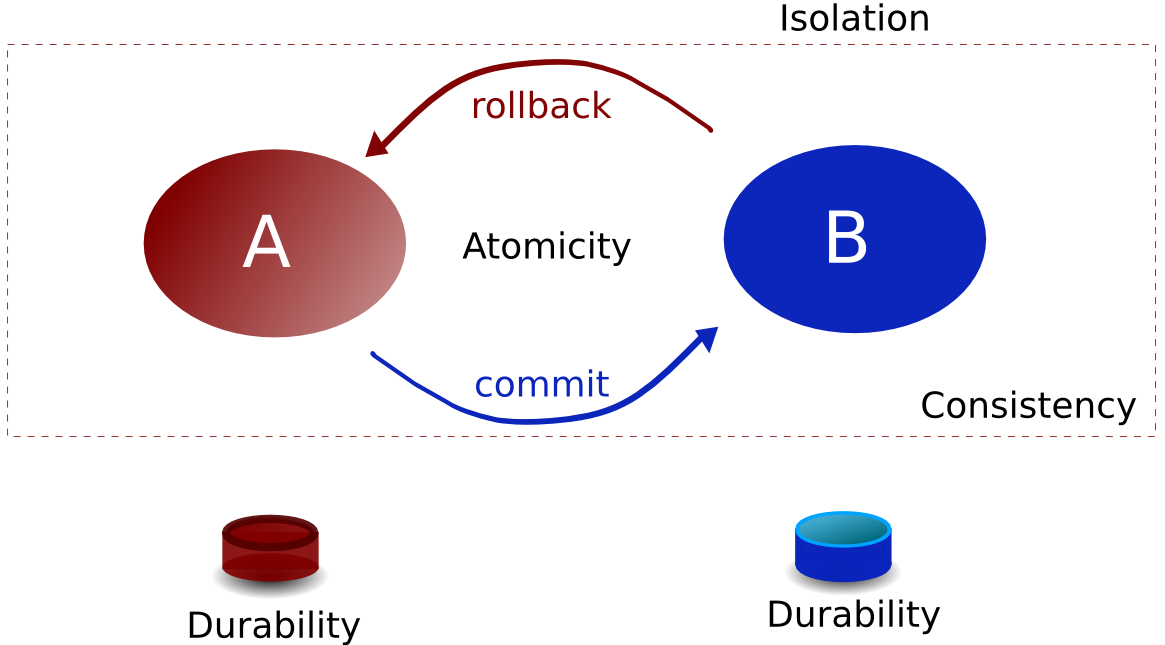
\includegraphics[scale=0.25]{img/transaction.png}
      \caption{Caractéristique d'une transaction}
      \label{tx}
    \end{center}
  \end{figure}
}

\ifslide{
  \begin{frame}{Transaction}
   \begin{center}
     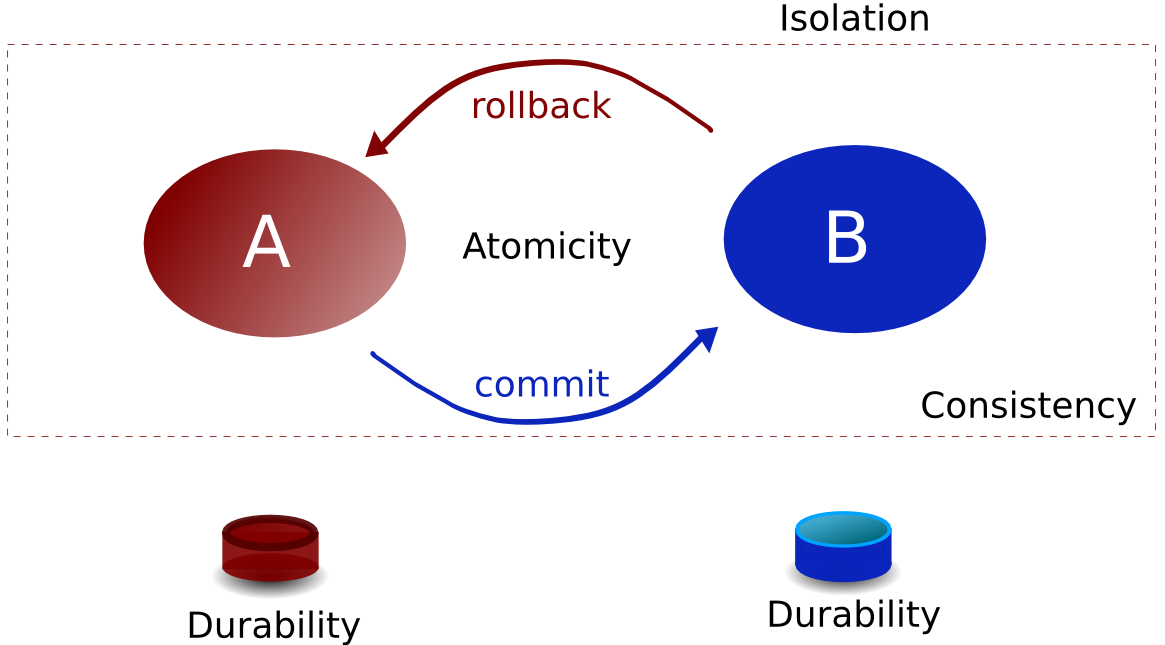
\includegraphics[scale=0.3]{img/transaction.png}
   \end{center}
  \end{frame}
}

\ifbook{

  \mysubsubsection{Atomicité des transactions}

  \paragraph{} L'aspect transactionnel de la plupart des opérations effectuées par un système
  informatique est un point important car c'est souvent à la charge du serveur d'applications ou du
  \textit{middleware} utilisé par l'application de l'assurer.

  \paragraph{} La caractéristique principale d'une transaction est son \textbf{atomicité}. En effet,
  à la fin de l'exécution d'une opération transactionnelle, on se retrouve soit dans un nouvel état
  (un \textbf{commit} a été effectué) ou dans l'état initial (un \textbf{rollback} a été réalisé).
  En outre, une transaction est très souvent une unité insécable, elle ne peut être découpée en
  plusieurs sous opérations distinctes, elle doit se réalise (ou non) au sein d'une opération, qui
  est donc atomique.
}

%% TODO: slide on tx isolation
\ifbook {

  \mysubsubsection{Isolation des transactions}

  \paragraph{} Les transactions s'exécutent la plupart du temps en parallèle les unes ou autres, il
  est donc crucial de correctement orchestrer ces opérations concurrentes pour s'assurer d'un
  résultat concurrent. C'est l'isolation d'une transaction qui garantit ce état cohérent.

  \paragraph{} L'isolation a pour conséquent concrète d'empêcher deux transactions de modifier de
  manière concurrente un objet. Si deux transactions concurrentes souhaitent modifier le même objet,
  l'une prendra la priorité et la seconde attendra la fin de cette dernière.

  \paragraph{} Un autre enjeu de l'isolation d'une transaction est de masqué les éventuels états
  intermédiaires obtenues lors de son exécution. À l'insu de la transaction, on se trouve dans
  l'état souhaité ou dans l'état initial, mais en aucun cas, dans un état intermédiaire.

  \paragraph{} Néanmoins, sérialiser systématiquement les transactions pose de gros problèmes de
  performances, et ce n'est donc pas toujours possibles. Certains systèmes, tel que la plupart des
  bases de données, utilise donc un système de contrôle actifs des opérations concurrentes, et
  n'isole donc pas leurs transactions.

  \paragraph{} On peut donc déjà noter qu'une transaction n'a que deux statuts de fin d'exécution
  possible:

  \begin{itemize}
    \item \textbf{commit}
    \item \textbf{rollback}
  \end{itemize}

  \begin{figure}[hb]
    \begin{center}
      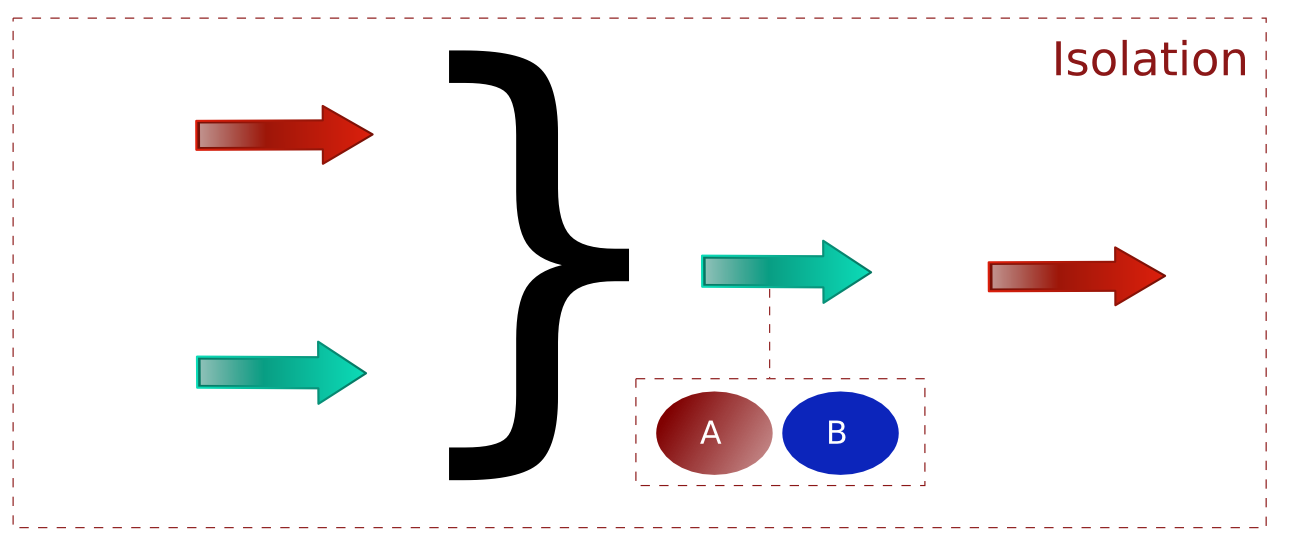
\includegraphics[scale=0.3]{img/tx-isolation.png}
      \caption{Isolation d'une transaction}
      \label{tx-isolation}
    \end{center}
  \end{figure}
}

\ifslide{
  \begin{frame}{Coût en performance d'une transaction}
   \begin{center}
     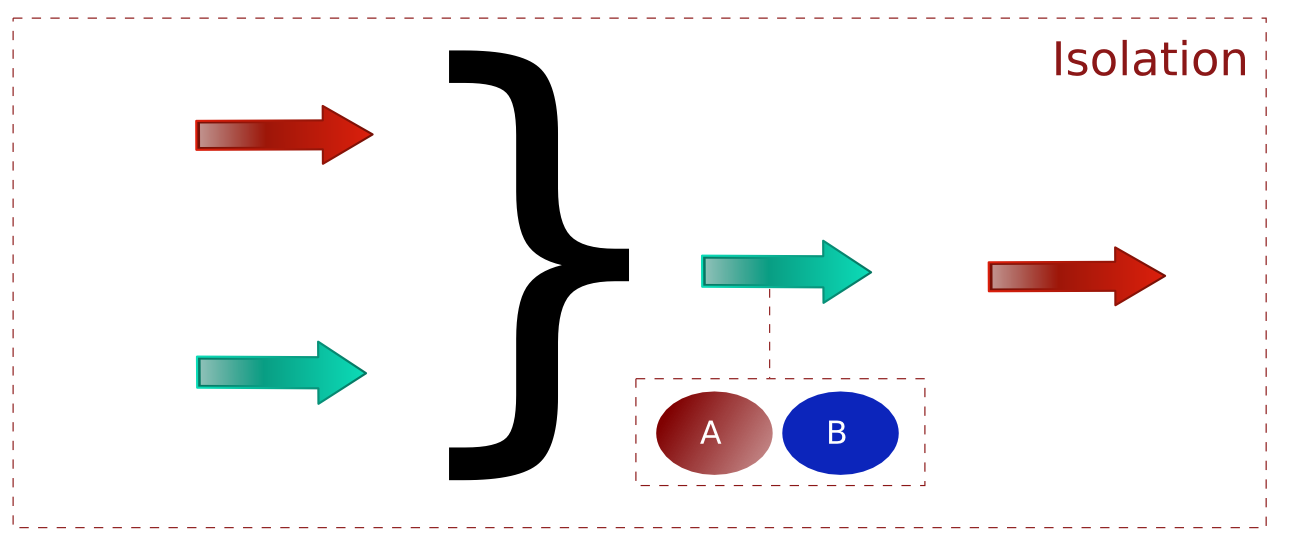
\includegraphics[scale=0.25]{img/tx-isolation.png}
   \end{center}
  \end{frame}
}

\ifbook {
  \mysubsubsection{Sémantique d'une transaction}

  \paragraph{} La théorie derrière la notion de transaction dispose, comme toute théorie, de sa
  propre sémantique, offrant un certain niveau d'abstraction. Pour décrire la réalisation d'une
  transaction, on désigne les différents systèmes entre en jeu sous les noms suivants:

  \begin{itemize}
    \item les \textbf{participants} sont les différents systèmes impliqués dans la transaction ;
    \item \textbf{coordinateur} est le système qui se charge de coordonner les participants.
  \end{itemize}

  \paragraph{} Plus concrètement, au début d'une transaction, le \textbf{coordinateur} demande à
  chaque \textbf{participants} si ils sont près à effectuer leur \textbf{commit}. Une fois que tous
  ont répondu de manière favorable, le coordinateur demande à tous d'effectuer l'opération, et
  retourne et l'état de \textbf{commit} est retourné.

  \paragraph{} Dans la théorie, bien évidemment, les participants sont garant de leur état, et, si
  ils s'engagent à pouvoir effectue leur \textbf{commit}, ils ne peuvent en aucun cas échoué par la
  suite. Dans la pratique, il est difficile de garantir une telle robustesse\footnote{Spécialement,
  pour garantir que leur opération soit ACID, les systèmes doivent pouvoir obtenir un
  \textbf{verrou} sur la ressource qu'il manipule, et, dans la pratique, c'est en fait très
  difficile à mettre en place...}.

  \paragraph{} Ce mécanisme de transaction est souvent désigné sous le nom de \textbf{two phase
  commit}. En effet, ce dernier se déroule en deux phases, une de préparation où chaque participants
  s'engagent (ou non) à effectuer un \textbf{commit}, et une seconde, où leur coordinateur déclenche
  l'exécution de ces opérations.

  \paragraph{} On notera que le protocole du \textbf{two phase commit} est très abstrait et ne
  préjuge en aucun cas d'une architecture logicielle ou physique. Le coordinateur, par exemple, peut
  s'exécuter au sein d'un même processus que la transaction ou être exécuté sur une autre physique.
}


%%TODO: slide on READ/WRITE, OPTIMIST/PESSIMIST

\ifbook{
  \subsubsection{Contrôle de la concurrence dans le "two phase commit"}

  \paragraph{} On peut simplifier les transactions exécutées par un système en deux catégorie : les
  transactions effectuant des opérations de lecture (\textbf{READ}) et celle d'écriture
  (\textbf{WRITE}). Il est évident que des opérations de lectures peuvent s'exécuter de manière
  concurrente sans nécessiter de verrou sur les données qu'elles accèdent.

  \paragraph{} À l'inverse, les opérations d'écriture nécessitent la mise en place d'un
  \textbf{verrou exclusif}. Ce dernier a pour rôle de bloquer d'éventuels autres opérations
  d'écriture que les opérations de lecture. En effet, ces dernières doivent accéder à un état cohérent, et
  non à un état intermédiaire, produit par l'opération d'écriture en cours d'exécution.

  \paragraph{} Pour optimiser ce fonctionnement, il existe deux \textbf{stratégies de
  verrouillage}\footnote{Il existe fait plus de stratégie, qui sont généralement des variations
  des deux présentés ici}:

  \begin{description}
    \item[Pessimiste] Cette stratégie part du principe que les opérations d'écritures concurrentes
    sont fréquentes, et opte donc pour utiliser systématiquement un verrou. En plus d'avoir un effet
    négatif sur les performances, cette stratégie augmente le risque d'apparition \textbf{deadlock} (que
    nous verrons plus loin), mais elle assure une forte cohérence des données obtenues.
    \item[Optimiste] Cette stratégie se fonde elle sur justement très peu d'opérations en écritures
    concurrentes et un très grand nombre d'opération en lecture. Pour assurer que ces derniers ne
    soient pas entraver par les opérations en écritures, ces dernières ne posent pas de verrou, et
    le système se contente d'effectuer un \textbf{rollback} en cas d'opération d'écriture
    concurrente.
  \end{description}
}

%% TODO: Slide on deadlock

\ifbook{

  \mysubsubsection{Deadlock}

  \paragraph{} Le principal intérêt des transactions réside dans la garantie sur la cohérence des
  données. En effet, l'utilisation de transactions assurent que si deux processus accèdent et
  modifient, de manière concurrente, la même donnée, l'une des opérations n'écrasera pas simplement
  le résultat de l'autre.

  \paragraph{} À ce regard, la transaction remplit un peu prêt le même rôle que le système
  d'exploitation dans l'arbitrage des accès aux données entre processus. Prenons un exemple
  simpliste, pour l'illustrer.

  \paragraph{} Si deux processus cherche à incrémenter une valeur A de manière concurrente,
  hors de toute transaction, le résultat A + 1, puisque lors de leur accès à la valeur, celle ci est
  égale à A, et que les deux requêtes de chaque processus, aboutit à l'enregistrement de la valeur A
  +1. En isolant ces opérations à l'aide de transactions, l'un des processus modifiera la valeur A
  à A + 1, pendant que le second devra attendra la fin de la transaction pour effectuer son
  opération. A l'issu des opérations, la valeur de la donnée est donc A + 2.

  \paragraph{} De manière similaire à la gestion de processus au sein d'un système d'exploitation,
  là aussi le risque de créer une situation de \textbf{deadlock}, où deux verrous se bloquent
  mutuellement, sont assez élevée. Il existe donc, dans la plupart des systèmes de gestions de
  transactions, des mécanismes pour détecter ces situations indésirables et en sortir.

  \paragraph{} La plupart des systèmes proposent l'une des deux stratégies de détection et
  résolution de \textbf{deadlock} suivantes (si ce n'est les deux):

  \begin{description}
    \item[\textit{timeout}] Cette stratégie, simple et robuste, consiste à poser une contrainte de
    temps, de l'ordre de quelques minutes la plupart du temps, selon l'exécution d'une transaction.
    Si cette dernière n'a pas fini de s'exécuter avant ce délais, elle est tout simplement avortée,
    et un \textbf{rollback} est effectué.
    \item[graphe] Une autre stratégie plus élaborée consiste à conserver un état du graphe formé par
    l'ensemble des transactions, et de le parcourir, pour détecter des situations de verrouillage.
    Ce mécanisme est bien évidemment beaucoup plus couteaux et complexe à mettre en place, mais
    permet d'assurer la détection, et la résolution, des situations de \textbf{deadlock} beaucoup
    plus rapidement.
  \end{description}
}

%% TODO: nested tx

\ifbook{
  \mysubsubsection{Nested transaction}

  \paragraph{} Moins souvent utilisée et rencontrée, les \textit{nested transaction} méritent
  néanmoins d'être brièvement mentionnées. Elles concevoir une transaction en encapsulant en son
  sein différents autres transactions (ou sans transactions).

  \paragraph{} L'avantage de cette stratégie est que l'on peut aisément rejouer une des sous
  transactions, si elle échoue - et non refaire l'ensemble de la transaction\footnote{On désigne
  ceci en anglais par le terme \textbf{isolation fault}}. En outre, l'aspect \textbf{durable} de la
  transaction n'est garanti que à la fin de l'exécution de la \textbf{top level transaction} et non
  des \textbf{nested transaction}.

  \paragraph{} La durabilité d'une transaction étant à la fois difficile à obtenir et coûteux en
  terme de performance, cette stratégie peut se révéler très pertinent dans l'optimisation d'un
  système.
}

%% TODO: implicit tx

\ifbook{
  \mysubsubsection{Transaction implicite}

  \paragraph{} Il est aussi important de souligner que même si l'application n'est pas
  transactionnel en tant que tel elle peut utiliser tout à fait utiliser des transactions de manière
  implicite. En effet, de nombreux services ou composant, justement issu du \textit{middleware}
  utilisé par l'application, peuvent tout à fait présenter des aspects transactionnel.

  \paragraph{} Prenons par exemple une application affichant sur un terminal sur un tableau. Elle se
  contente d'effectuer, à intervalles régulier, une opération de sélection sur la table d'une base
  de données et elle n'effectue aucune opération en écriture. En première analyse, il n'y a aucune
  raison pour que l'application soit transactionnel.

  \paragraph{} Elle ne l'est pas, mais elle utilise néanmoins une source de données sur laquelle
  elle effectue des requêtes SQL, qui, elles, sont transactionnelles. Ainsi, pour peu que
  l'application utilise, par ailleurs, un autre \textit{middleware}, lui aussi transactionnel, on
  peut se retrouver face à des problématiques d'isolation ou de \textit{deadlock}, sans que
  l'application métier soit, en tant que tel, transactionnel.
}

\ifbook{
  \mysubsubsection{Coût des transactions}

  \paragraph{} Si effectuer une opération au sein d'une transaction apporte de grande avantage, il
  va s'en dire qu'elle s'accompagne de grandes contraintes et surtout d'un coût certain en terme de
  performance. En effet, sur l'extrait de code suivant, il est aisé d'estimer laquelle des deux
  méthodes est la plus rapide à s'exécuter:

  \begin{figure}[hb]
    \begin{center}
      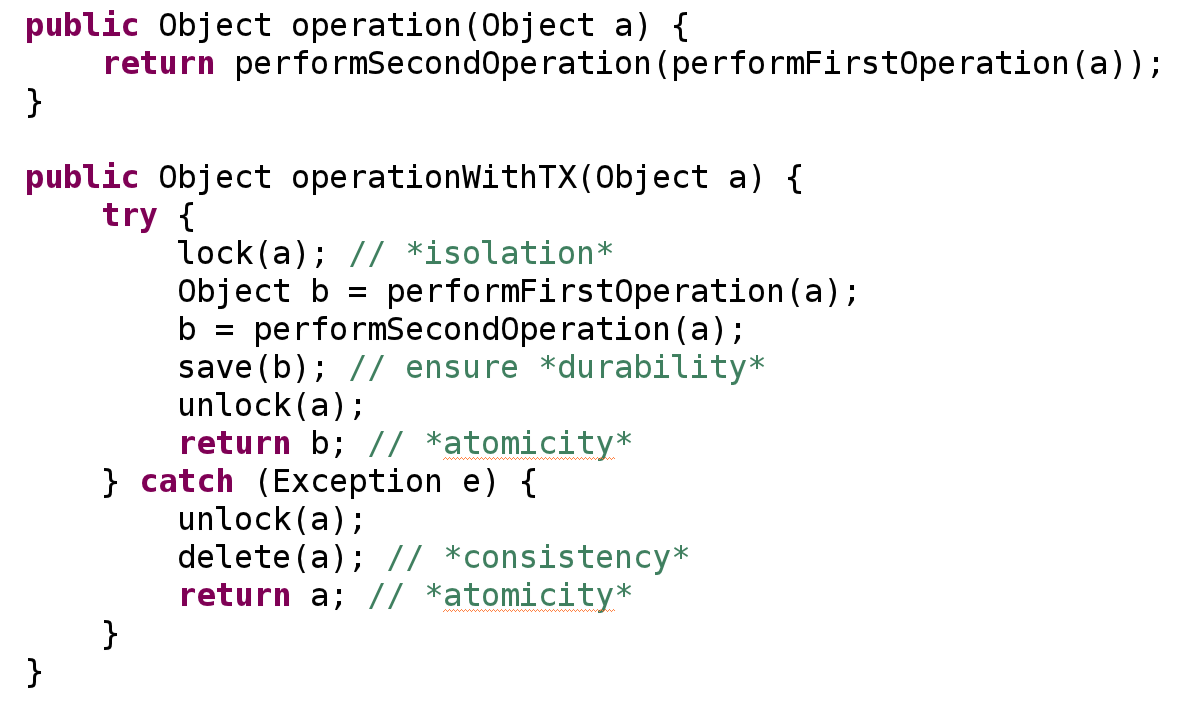
\includegraphics[scale=0.4]{img/transaction-cost.png}
      \caption{Coût en performance d'une transaction}
      \label{tx-cost}
    \end{center}
  \end{figure}

  \paragraph{} Le pseudo code présenté \ref{tx-cost} (page \pageref{tx-cost} n'est fourni
  qu'à titre d'exemple pédagogique. Lors de la mise en place de transaction au sein d'une
  application, le conteneur d'exécution, qu'il s'agisse d'une machine virtuelle ou du serveur
  d'application, fournit une API appropriée.

  % TODO Utilisé l'API et montrer les capacités de monitoring associé ?
}

\ifslide{
  \begin{frame}{Coût en performance d'une transaction}
   \begin{center}
     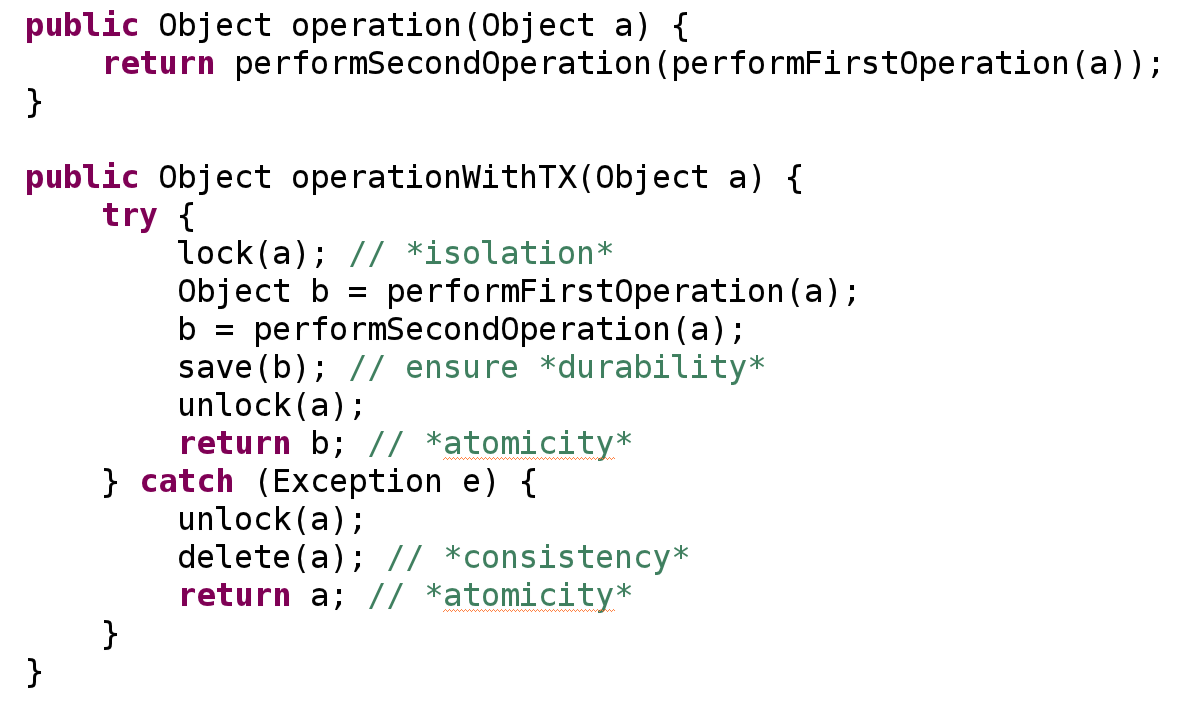
\includegraphics[scale=0.25]{img/transaction-cost.png}
   \end{center}
  \end{frame}
}

\ifbook{
  \mysubsubsection{Être (transactionnelle) ou ne pas être (transactionnel) ?}

  \paragraph{} Il est donc bien important, lors de la conception d'une application, de bien
  réfléchir à la nécessité ou non d'utiliser des transactions. Une preuve très flagrante de ceci est
  l'émergence des bases de données non transactionnel.

  \paragraph{} Avec l'augmentation des applications "web", mais surtout de leurs nombres
  d'utilisateurs, les bases de données relationnelles deviennent généralement le goulot
  d'étranglement. Comme évoqué précédemment, chaque requête vers ces base de données sont en effet
  des transactions exigeant, dans chaque tiers, un certains travail supplémentaire. En supprimant
  l'aspect transactionnel des échanges entres l'application et la source de données, ces bases de
  données offrent de bien meilleur performance.

  \paragraph{} Bien évidement, on s'expose aussi à des nombreux problèmes de corruption ou pertes de
  données, mais, il existe des applications où ce genre de situation est plus supportable qu'une
  perte de performance.

  \paragraph{} Par exemple, pour un jeu en ligne, que le tableau donnant la liste des 10 dernières
  meilleurs scores ne soit pas toujours cohérent et qu'il soit même parfois corrompu n'est pas un
  réel problème. A l'inverse, un le jeu qui devient trop lent, juste parce que les accès au tableau
  des meilleurs scores ralentit l'application, est un réel problème.
}
